\documentclass[10pt,a4paper,spanish]{article}

\usepackage[spanish]{babel}
\usepackage[utf8]{inputenc}
\usepackage{amsmath, amsthm}
\usepackage{amsfonts, amssymb, latexsym}
\usepackage{enumerate}
\usepackage[official]{eurosym}
\usepackage{graphicx}
\usepackage[usenames, dvipsnames]{color}
\usepackage{colortbl}
\usepackage{multirow}
\usepackage{fancyhdr}
\usepackage[all]{xy}
\usepackage[below]{placeins}
\usepackage{subfigure}
\usepackage{eso-pic}
\usepackage{minted}
\usepackage{hyperref}
\usepackage[spanish]{algorithm2e}
\usepackage[a4paper]{geometry}
\geometry{top=2.5cm, bottom=2.5cm, left=3cm, right=3cm}

\hypersetup{
    colorlinks,
    citecolor=blue,
    filecolor=blue,
    linkcolor=black,
    urlcolor=blue
}
\phantomsection
\setlength\parindent{0pt}
\newcommand\BackgroundPic{
\put(0,0){
\parbox[b][\paperheight]{\paperwidth}{%
\vfill
\centering
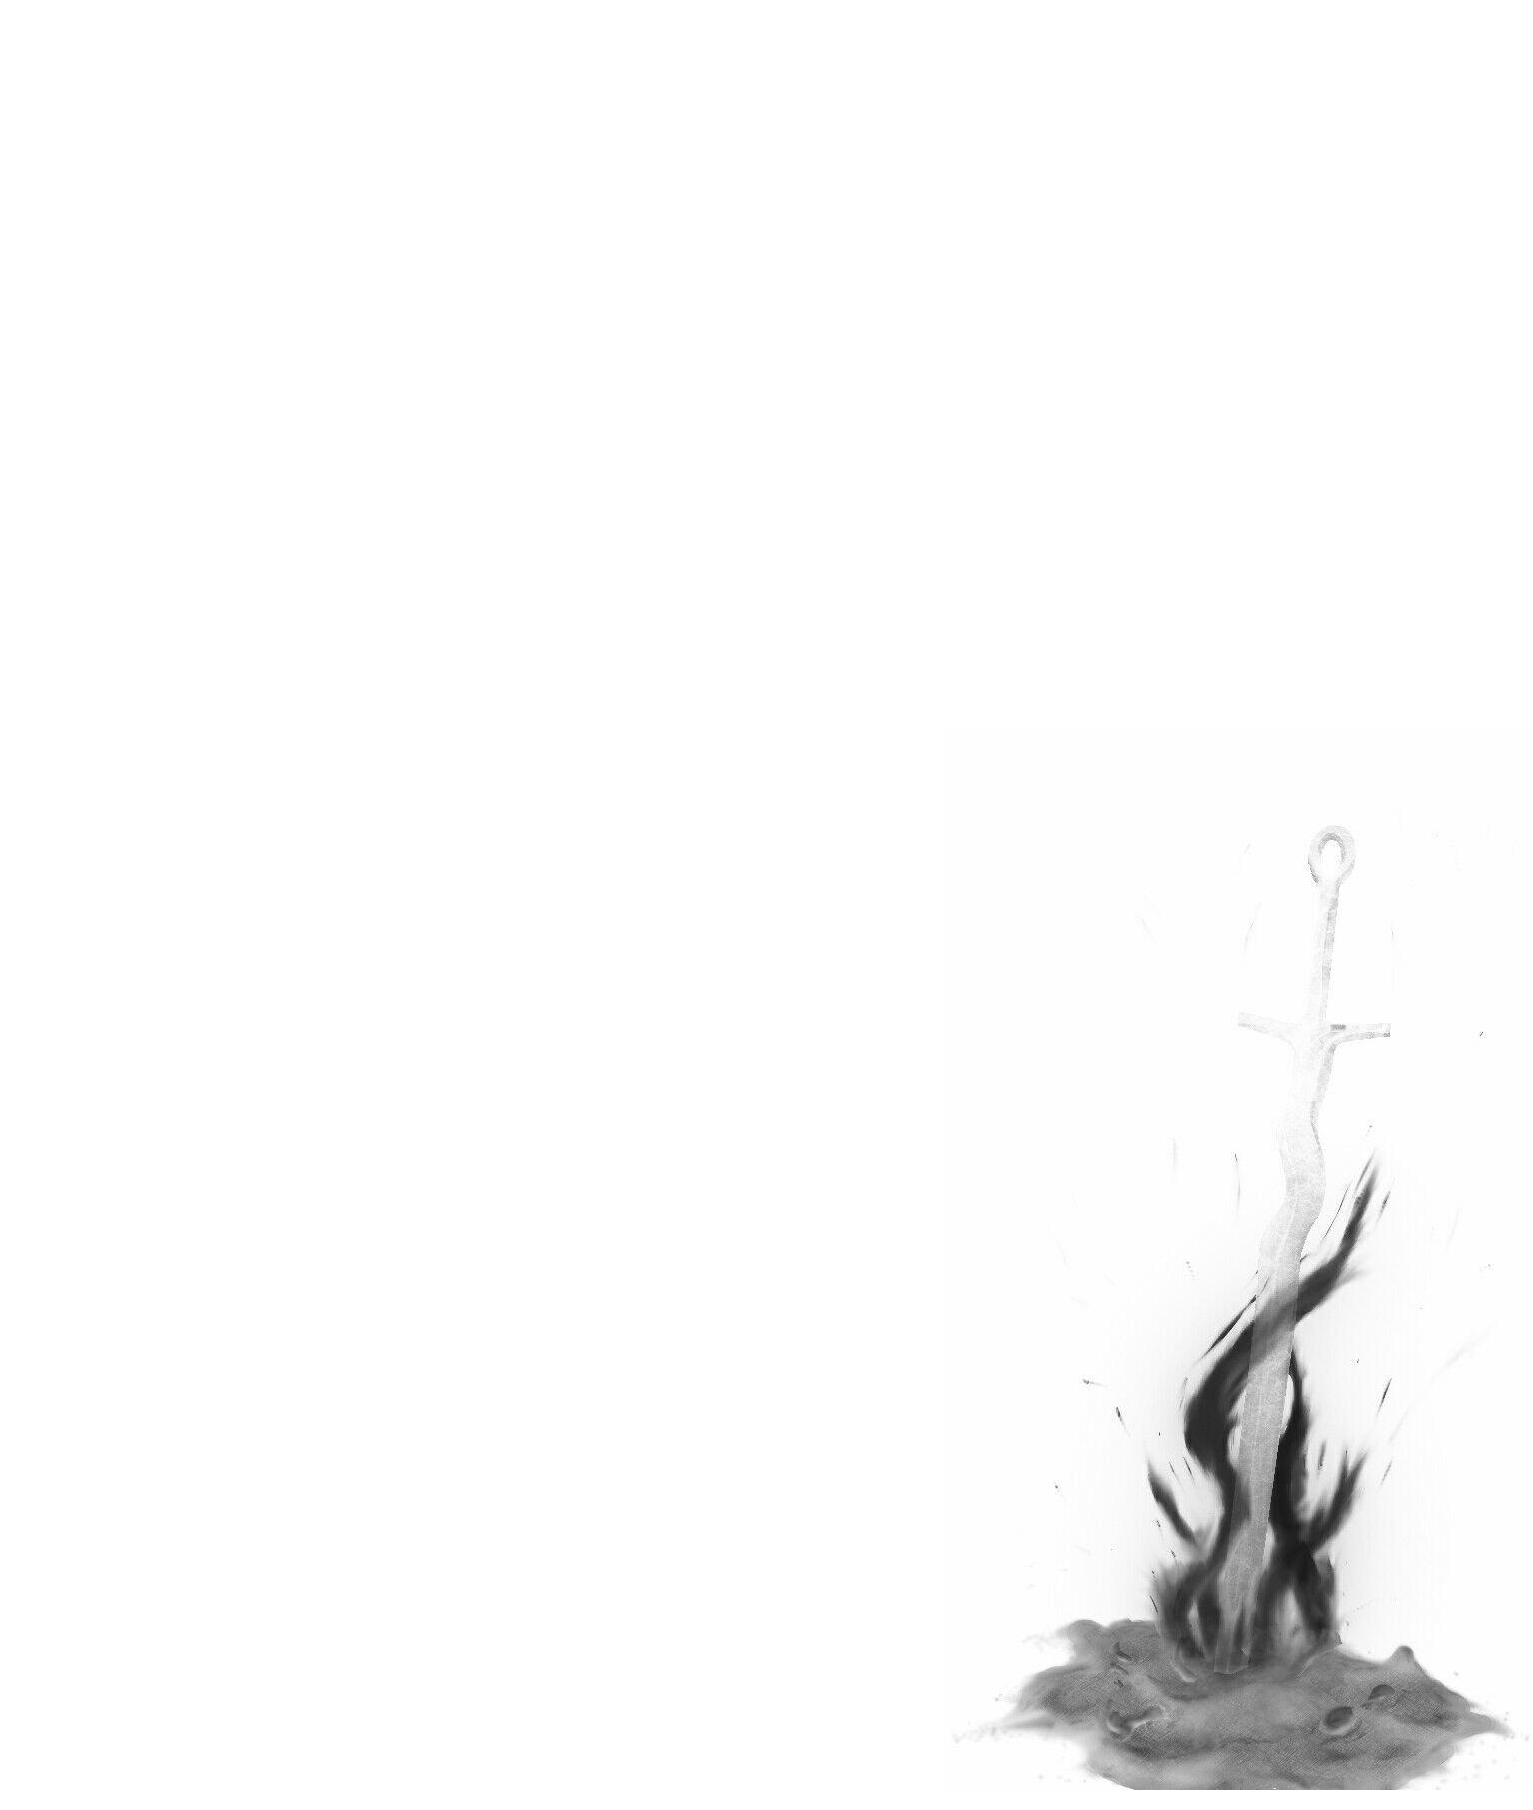
\includegraphics[width=\paperwidth,height=\paperheight,
keepaspectratio]{../Imagenes/bonfire} %cambiad la ruta a la foto de background
\vfill
}}}

\DeclareGraphicsExtensions{.png,.pdf,.jpg,.gif }



\title{Título}
\date{\today}

\begin{document}

\AddToShipoutPicture{\BackgroundPic}

\begin{titlepage}

\begin{center}
\vspace*{-1in}
\begin{figure}[htb]
\begin{center}

\includegraphics[width=8cm]{../Imagenes/portada} %cambiad la ruta a la foto de portada
\end{center}
\end{figure}

ESCUELA TÉCNICA SUPERIOR DE INGENIERÍA INFORMÁTICA Y TELECOMUNICACIONES\\
\vspace*{0.15in}
\vspace*{0.2in}
Asignatura\\
\vspace*{0.6in}
\rule{80mm}{0.1mm}\\
\vspace*{0.2in}
\begin{Large}
\textbf{Título} \\
\end{Large}
\vspace*{0.3in}
\begin{large}
Documentacion a \LaTeX{}\\
\end{large}
\vspace*{0.3in}
\rule{80mm}{0.1mm}\\
\vspace*{0.1in}
\begin{large}
Hecho por: \\
Autor\\
\end{large}
\end{center}

\end{titlepage}

\AddToShipoutPicture{\BackgroundPic}

\tableofcontents
\listoffigures

% \maketitle



% Ejemplo de como insertar fotocon el caption para el índice de figuras
% \begin{figure}[H] %con el [H] le obligamos a situar aquí la figura
% 	\centering
% 	\includegraphics[scale=0.3]{{image.jpg}}  %el parámetro scale permite agrandar o achicar la imagen. En el nombre de archivo puede especificar directorios
% 	\label{figura1}
% 	\caption{captacion}
% \end{figure}

\newpage


% Bibliografía, para acceder a ella es necesario usar \cite{Lo que hay dentro de \bibitem}
\begin{thebibliography}{X}
  \bibitem{Bibliografia} \textsc{Title} \url{http://www.referencia.com}
\end{thebibliography}

\newpage
\ClearShipoutPicture


\end{document}
